\section{Free Research}

In this part we had some freedom to put some creativity to work, for that we tried to search for some specific surgery to implement. When we were doing some research, come to our minds that we could do an app to test different "surgeries". For that we used the "app designer" from matlab to create the app. 

This app asks for some values relative to the robot's dimension, pose, the gains, the organ's place, dimension and the trajectory needed to be done by the robot. To test this part, it's only needed to start the main file, write the numbers for the test (the values for the pose needs to be in radians, like pi/2) and finally click the start button to get the surgery test.

\begin{figure}[H]
    \centering
    \includegraphics[width=0.49\textwidth]{imgs/f3.png}
    \caption{App for the tests}
    \label{fig:f3}
\end{figure}

The figure \ref{fig:f3} is the app that we developed, where we need to write the values we want to use are (l1,l2,l3-dimensions of the robot; q1,q2,q3-pose of the robot; center-x,center-y,radius-values for the vital area; Kp,Kq-proportional gain and the force given to the vital area to keep the robot away; x0,y0,mx,my-values for the trajectory. 

The simulink is the same as before, as in the exercise about trajectory design. Using this app we can change a lot of variants in these tests, we can change values about the robot, about the trajectory and even about the vital area that we want to use. This app was developed as a way to test different situations in surgeries, it can test if the robot behaves as it is supposed and also if the pose given to the robot is good enough so it can do well the trajectory. 

We did some tests to see if the app is running good, but there is a lot of other tests that can be done.

\begin{figure}[H]
    \centering
    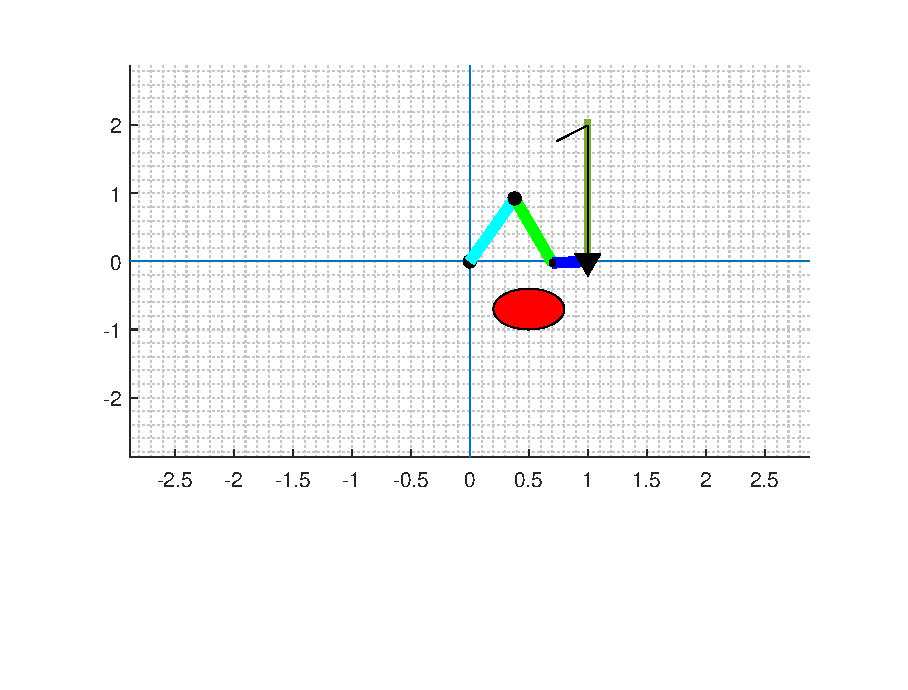
\includegraphics[width=0.49\textwidth]{imgs/f1.eps}
    \caption{App for the tests}
    \label{fig:f1}
\end{figure}

\begin{figure}[H]
    \centering
    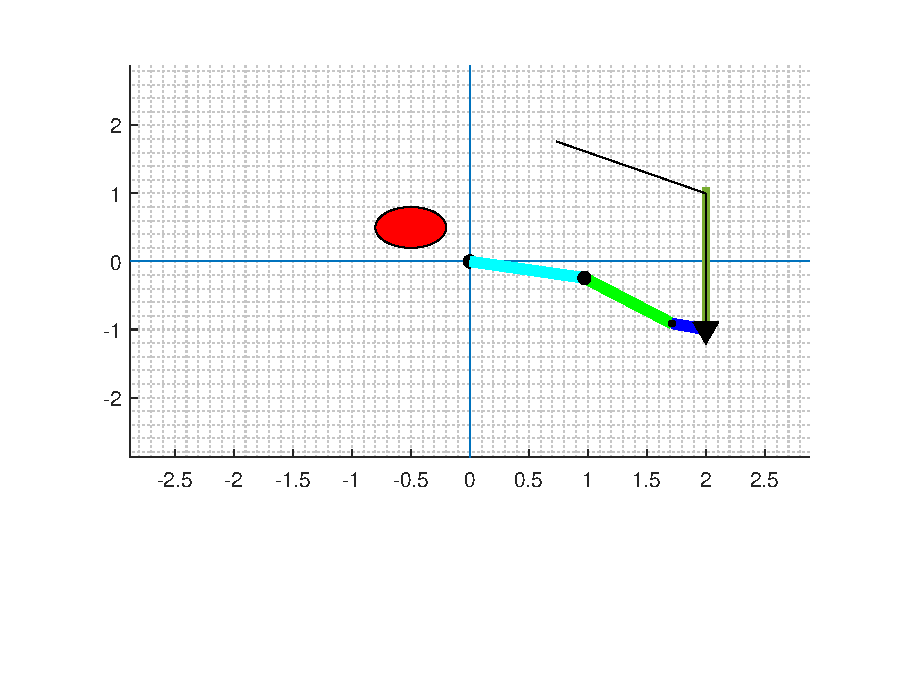
\includegraphics[width=0.49\textwidth]{imgs/f2.eps}
    \caption{App for the tests}
    \label{fig:f2}
\end{figure}

We can see in the examples, well done trajectories and in the Figure \ref{fig:f1} the robot has to change it's pose to not touch the vital are.
For the tests we used the next values:

Figure \ref{fig:f1}
\begin{itemize}
    \item l1=1;l2=1;l3=0.3
    \item q1=pi/5;q2=pi/4;q3=pi/3
    \item center-x=0.5;center-y=-0.7;radius=0.3
    \item kp=100;kq=10;
    \item mx=0;my=-1.5;x0=1;y0=1
\end{itemize}

Figure \ref{fig:f2}
\begin{itemize}
    \item l1=1;l2=1;l3=0.3
    \item q1=pi/5;q2=pi/4;q3=pi/3
    \item center-x=-0.5;center-y=0.5;radius=0.3
    \item kp=100;kq=10;
    \item mx=0;my=1;x0=2;y0=0
\end{itemize}

Concluding, we think that this app can help to predict if a surgery would succeed or not by testing here before, with the values from the robot, the vital area and the trajectory.